\documentclass{article}
\oddsidemargin=0in
\topmargin=-0.5in
\textwidth=6.5in
\textheight=9in

\title{\vspace{-25mm}MATH 440: Assignment 2\vspace{-2.5mm}}
\author{Josh Manis}
\date{\vspace{-2.5mm}Due: March 22, 2018}

\usepackage[margin=2.5cm]{geometry}
\usepackage{titling}
\usepackage{enumerate}
\usepackage{amsmath, amssymb, mathtools, commath, amsfonts, amsthm}
\usepackage{graphicx, float, color, xcolor}
\usepackage{listings, booktabs}
\usepackage{color}
\usepackage{etoolbox}
\usepackage{braket}
\usepackage{easybmat}
\usepackage{tikz, pgfplots}
\usepackage{breqn}
\usetikzlibrary{matrix, calc, patterns, positioning, shapes}

\everymath{\displaystyle}
\newcommand{\Z}{\ensuremath{\mathbb{Z}}}
\newcommand{\N}{\ensuremath{\mathbb{N}}}
\newcommand{\Q}{\ensuremath{\mathbb{Q}}}
\newcommand{\R}{\ensuremath{\mathbb{R}}}
\newcommand{\A}{\ensuremath{\mathrm{A}}}
\newcommand{\B}{\ensuremath{\mathrm{B}}}
\newcommand{\C}{\ensuremath{\mathrm{C}}}
\newcommand{\X}{\ensuremath{\mathrm{X}}}
\newcommand{\Y}{\ensuremath{\mathrm{Y}}}

\newtheorem*{thm*}{Theorem}
\theoremstyle{remark}
\newtheorem*{prop*}{Proposition}
\newtheorem*{lem*}{Lemma}
\theoremstyle{remark}
\newtheorem{case}{Case}

\newcommand{\diff}[2]{\frac{\dif#1}{\dif#2}}
\newcommand{\codom}[1]{\mathrm{codom}\left(#1\right)}
\newcommand{\Mod}[1]{\ \left(\mathrm{mod}\ #1\right)}
\newcommand{\sunderline}[1]{\underline{\smash{#1}}}
\newcommand{\p}{\phantom{-}}
\newcommand{\numberthis}{\addtocounter{equation}{1}\tag{\theequation}}
\renewcommand{\qed}{\hfill\ensuremath{\blacksquare}}
\renewcommand{\epsilon}{\varepsilon}
\newcommand{\TODO}{\emph{\underline{\textbf{DO THIS AT SOME POINT}}}}
\lstset{
	columns=flexible,
	basicstyle=\small\ttfamily,
	mathescape=false,
	escapeinside=||,
}

\makeatletter
\patchcmd\start@gather{$$}{%
	$$%
	\displaywidth=\textwidth
	\displayindent=-\leftskip
}{}{}
\patchcmd\start@align{$$}{%
	$$%
	\displaywidth=\textwidth
	\displayindent=-\leftskip
}{}{}
\patchcmd\start@multline{$$}{%
	$$%
	\displaywidth=\textwidth
	\displayindent=-\leftskip
}{}{}
\patchcmd\mathdisplay{$$}{%
	$$%
	\displaywidth=\textwidth
	\displayindent=-\leftskip
}{}{}
\makeatother

\makeatletter
\g@addto@macro\@floatboxreset\centering
\makeatother

\pretitle{\begin{flushright}}
\posttitle{\end{flushright}}
\preauthor{\begin{flushright}}
\postauthor{\end{flushright}}
\predate{\begin{flushright}}
\postdate{\end{flushright}}


\begin{document}
	\maketitle
	
	The goal of this assignment was to approximate the definite integral of a highly oscillatory function on an interval of the real number line through difference methods using parallel computing. Let $K\in\{100,101,\dots,10000\}$ be a fixed wavenumber and $f(K,\cdot)\::\:[0,\pi]\subset\R\mapsto\R$, then define
	\begin{align*}
		H(K)&:=\int_{0}^{\pi}f(K,x)\dif x\approx\sum_{i=1}^{K}\int_{a_i}^{b_i}f(K,x)\dif x\approx\sum_{i=1}^{K}A(K,i),
		\intertext{where $A(K,i)$ is an approximation to the partial integral of $f(K,\cdot)$ on $[a_i,b_i]\subset\R$ of width $\pi/K$. Now take 101 quadrature points, $x_{i,j}$, on $[a_i,b_i]$, in order to compute $A(K,i)$ using the midpoint method, $A_{M,101}(K,i)$, the trapezoid method, $A_{T,101}(K,i)$, and Simpson's method, $A_{S,101}(K,i)$, where}
		a_i&=x_{i,0}<x_{i,1}<\cdots<x_{i,100}<x_{i,101}=b_i, \\
		\xi_{i,j}&=\frac{x_{i,j-1}+x_{i,j}}{2}, \\
		h_{i,j}&=x_{i,j}-x_{i,j-1}, \\
		A_{M,101}(K,i)&:=\sum_{j=1}^{101}f\left(K,\xi_{i,j}\right)h_{i,j}, \\
		A_{T,101}(K,i)&:=\sum_{j=1}^{101}\frac{1}{2}\left[f\left(K,x_{i,j-1}\right)+f\left(K,x_{i,j-1}\right)\right]h_{i,j}, \\
		A_{S,101}(K,i)&:=\frac{2}{3}A_{M,101}(K,i)+\frac{1}{3}A_{T,101}(K,i), \\
		&i\in\{1,2,\dots,K\},\:j\in\{1,2,\dots,101\}.
	\end{align*}
	The above was achieved with a main file and a module written in Fortran 90 compiled with mpif90. The code is as follows: \par
	\begin{figure}[H]\centering
		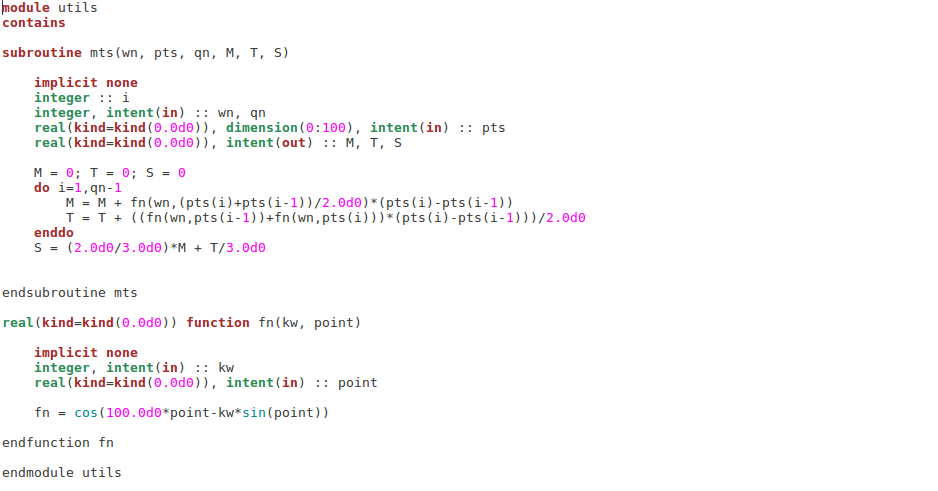
\includegraphics[scale=0.4]{mod.png}
	\end{figure}
	\begin{figure}[H]\centering
		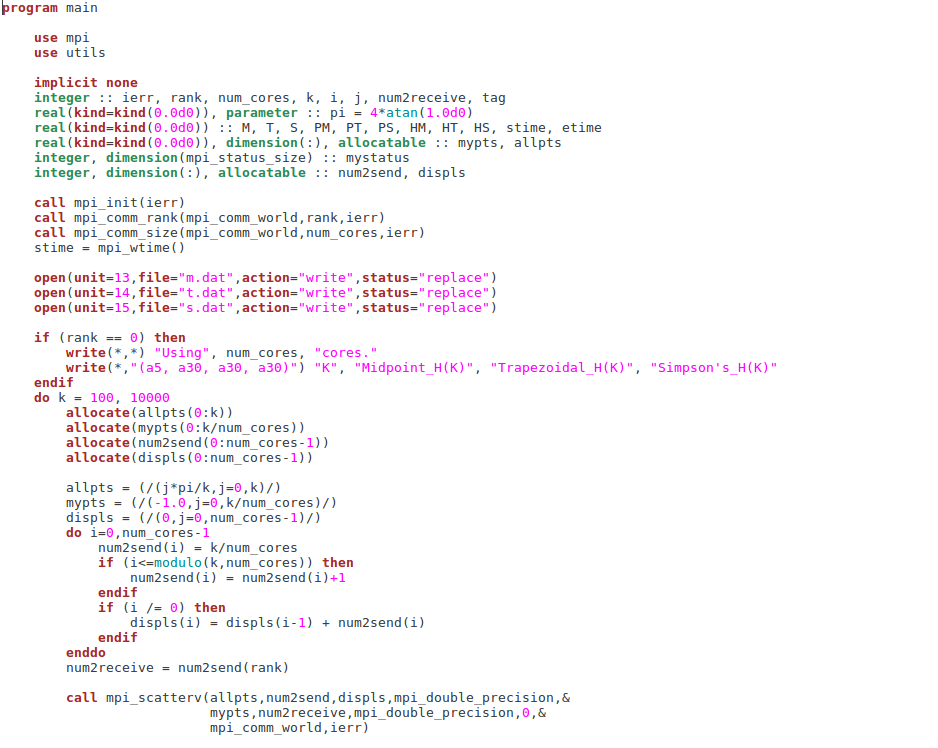
\includegraphics[scale=0.4]{main1.png}
	\end{figure}
	\begin{figure}[H]\centering\vspace{-5mm}
		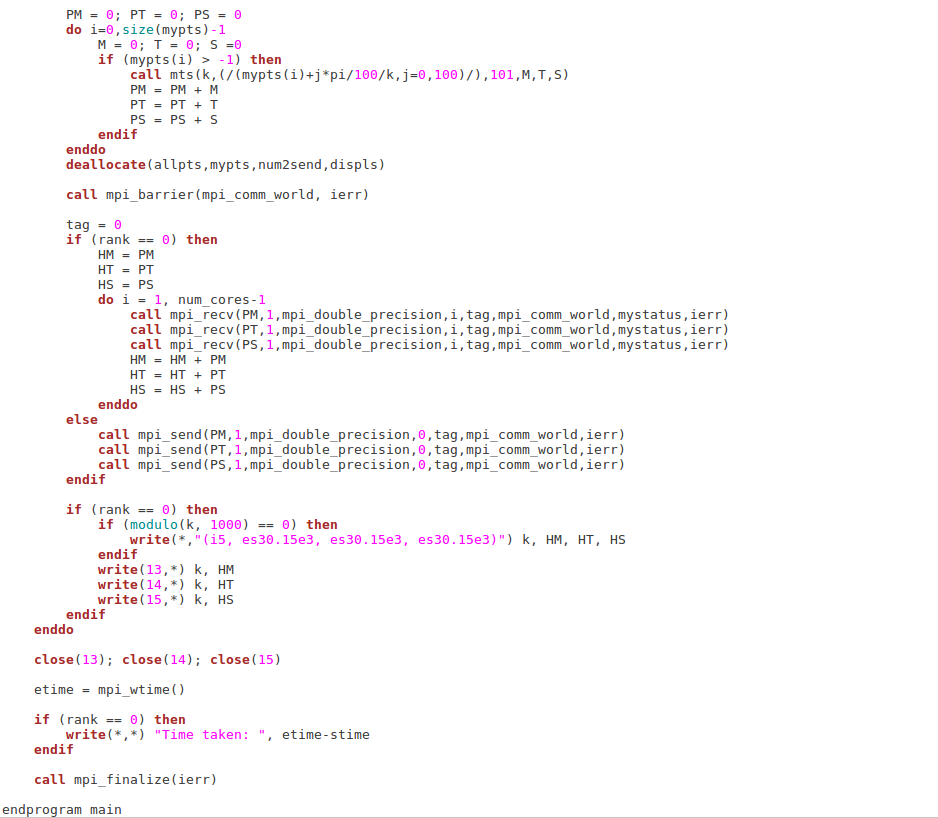
\includegraphics[scale=0.4]{main2.png}
	\end{figure}
	Running the above program will compute $H(K)$ for all $K\in\{100,101,\dots,10000\}$, writing output to the console when $1000\mid K$ and writing all values of $H(K)$ to a file. Some computed values using 8 cores are as follows: \par
	\begin{table}[H]
		\begin{tabular}{cccc}
			\toprule[0.5mm]
			 $K$  &        $H_{Mid}(K)$       &       $H_{Trap}(K)$       &       $H_{Simp}(K)$       \\
			\midrule
			 1000 & \p 3.819159292450652E-002 & \p 3.819146669047201E-002 & \p 3.819155084649498E-002 \\
			 2000 &   -4.844391641984440E-002 &   -4.844393643020983E-002 &   -4.844392308996622E-002 \\
			 3000 &   -3.642203217829408E-002 &   -3.642200581893822E-002 &   -3.642202339184213E-002 \\
			 4000 &   -1.417394345379661E-002 &   -1.417389887290094E-002 &   -1.417392859349807E-002 \\
			 5000 & \p 1.237969805213174E-002 & \p 1.237974211425157E-002 & \p 1.237971273950503E-002 \\
			 6000 & \p 2.957259450025162E-002 & \p 2.957262597415612E-002 & \p 2.957260499155312E-002 \\
			 7000 & \p 2.671023841147271E-002 & \p 2.671025176115547E-002 & \p 2.671024286136696E-002 \\
			 8000 & \p 6.324420119174937E-003 & \p 6.324415852441528E-003 & \p 6.324418696930464E-003 \\
			 9000 &   -1.641023755211308E-002 &   -1.641025431321439E-002 &   -1.641024313914685E-002 \\
			10000 &   -2.484826969529740E-002 &   -2.484829140135555E-002 &   -2.484827693065011E-002 \\		  
			\bottomrule[0.5mm]
		\end{tabular}
	\end{table}
	Some computed values using 16 cores are as follows: \par
	\begin{table}[H]
		\begin{tabular}{cccc}
			\toprule[0.5mm]
			 $K$  &        $H_{Mid}(K)$       &       $H_{Trap}(K)$       &       $H_{Simp}(K)$       \\ 
			\midrule
		 	 1000 & \p 3.462382957648013E-002 & \p 3.462385379110549E-002 & \p 3.462383764802190E-002 \\
			 2000 &   -4.837051599804793E-002 &   -4.837054657167911E-002 &   -4.837052618925834E-002 \\
			 3000 &   -3.644134234250336E-002 &   -3.644134045213760E-002 &   -3.644134171238143E-002 \\
			 4000 &   -1.392567124702175E-002 &   -1.392564881449324E-002 &   -1.392566376951225E-002 \\
			 5000 & \p 1.336853847205303E-002 & \p 1.336853524529409E-002 & \p 1.336853739646673E-002 \\
			 6000 & \p 2.958710956778173E-002 & \p 2.958714345406040E-002 & \p 2.958712086320795E-002 \\
			 7000 & \p 2.713810248334630E-002 & \p 2.713810085494336E-002 & \p 2.713810194054531E-002 \\
			 8000 & \p 6.025862388101258E-003 & \p 6.025892103065393E-003 & \p 6.025872293089307E-003 \\
			 9000 &   -1.674350874433848E-002 &   -1.674350783603062E-002 &   -1.674350844156919E-002 \\
			10000 &   -2.521455576408334E-002 &   -2.521453767524605E-002 &   -2.521454973447090E-002 \\
			\bottomrule[0.5mm]
		\end{tabular}
	\end{table}
	Something to note is that the computed values depend on the number of cores used. This is probably not good and is because of the way the subintervals are created and scattered to the cores. In order to compute the integral, the program creates $K$ starting points, one for each of the $K$ subintervals, $\left\{0,\frac{\pi}{K},\frac{2\pi}{K},\cdots,\frac{(K-1)\pi}{K}\right\}$. These starting points are then scattered, using \verb!mpi_scatterv!, to each of the cores in a balanced way. The cores then loop through their starting points and evaluate an integral by creating 101 quadrature points for each starting point, $\left\{\frac{i\pi}{K},\frac{i\pi}{K}+\frac{\pi}{100K},\cdots,\frac{(i+1)\pi}{K}\right\}$. Each core calculates a partial sum in this way and then all of the partial sums are collected, using \verb!mpi_recv! and \verb!mpi_send!, by the master core which calculates the full sum. Calculation time is then calculated using \verb!mpi_walltime!. By running the program with different numbers of cores, the complexity of the program can be determined. Time taken by number of cores used is as follows: \par
	\begin{table}[H]
		\begin{tabular}{cc}
			\toprule[0.5mm]
			Number of Cores & Time to Compute (s) \\ 
			\midrule
			 1 & 572.56358560398803 \\
			 2 & 303.70187161699869 \\
			 4 & 170.86698438599706 \\
			 8 & 92.290132593014278 \\
			16 & 49.949442379001994 \\
			32 & 30.678848117997404 \\
			\bottomrule[0.5mm]
		\end{tabular}
	\end{table}
	On average, doubling the amount of cores used, decreases the amount of time taken by a factor of $1.8$, this suggests that the complexity for this program is linear. The values of $H(K)$ and $K$ for $K\in\{100,101,\dots,10000\}$ were then graphed using \verb!gnuplots!, these graphs are shown below: \par
	\begin{figure}[H]\centering
		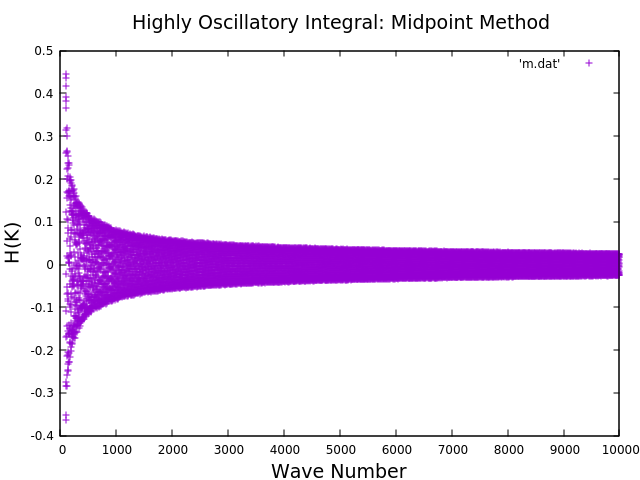
\includegraphics[scale=0.4]{m.png}
	\end{figure}
	\begin{figure}[H]\centering
		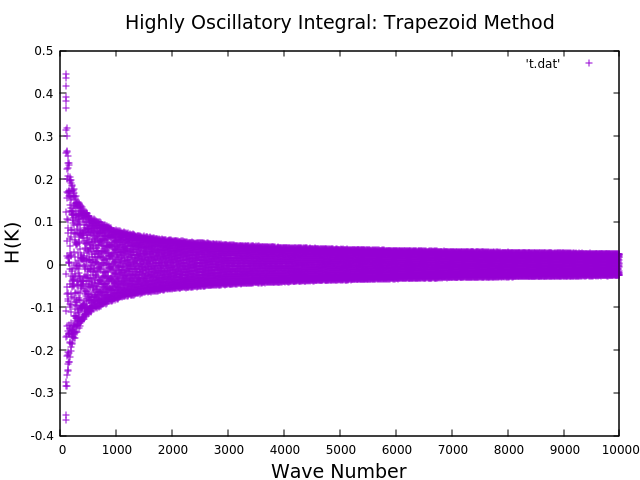
\includegraphics[scale=0.4]{t.png}
	\end{figure}
	\begin{figure}[H]\centering
		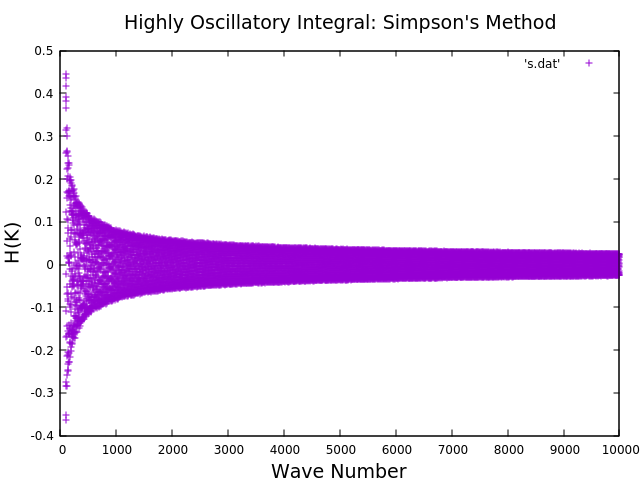
\includegraphics[scale=0.4]{s.png}
	\end{figure}
	We see that as $K$ grows large the value of $H(K)$ appears to be approaching $0$. This makes sense as we are calculating the integral of $\cos$ on $[0,\pi]$.
	
\end{document}


